\documentclass[../report.tex]{subfiles}
\begin{document}
\section{Annexes}
\subsection{Lien du projet}\label{subsec:projectlink}
Le projet est disponible sur le GitLab de l'école à l'adresse suivante :\\
\href{https://gitlab.forge.hefr.ch/frederic.bapst/prolog-truffle}{https://gitlab.forge.hefr.ch/frederic.bapst/prolog-truffle}\\
(une demande d'accès à monsieur Bapst est nécessaire)
\subsection{Librairies utilisées}
Cette section liste les différentes librairies nécessaires au fonctionnement du projet.
\subsubsection*{JLine3}
JLine est une librairie open source permettant de faciliter la gestion du terminal et de l'entrée utilisateur. Elle est utilisée jusqu'à la phase 2.\\
Lien : \href{https://github.com/jline/jline3}{https://github.com/jline/jline3}
\subsubsection*{ANTLR}
ANTLR est la librairie open source utilisée pour la réalisation du parser et du lexer. Elle a été utilisée durant tout le projet.\\
Lien : \href{https://github.com/antlr/antlr4}{https://github.com/antlr/antlr4}
\subsubsection*{JUnit}
JUnit est la librairie open source utilisée pour la réalisation des tests unitaires.\\
Lien : \href{https://github.com/junit-team/junit5/}{https://github.com/junit-team/junit5/}
\subsubsection*{Suite de librairies GraalVM et Truffle}
Truffle et les autres librairies de GraalVM sont utilisées pour l'implémentation du langage. Elles sont open source.\\
Lien : \href{https://github.com/oracle/graal}{https://github.com/oracle/graal}
\renewcommand{\thesubsection}{\Alph{subsection}}
\setcounter{subsection}{0}
\includepdf[angle=90, offset=2.1cm -0.1cm, pagecommand=\subsection{Planning}\label{subsec:planning}]{../../specs/planning.pdf}
\includepdf[pages={2}, offset=0 -2.5cm, pagecommand=\subsection{Manuel d'installation et d'utilisation}\label{subsec:manual}]{../../manual/manual.pdf}
\includepdf[pages={3-}]{../../manual/manual.pdf}
\end{document}